\section{\texorpdfstring{\GL}{GL}: A Logic for the Global Calculus}\label{Logic4Struct:sec:globalLogic}

In this section, we introduce a logic for choreography.  The logical language comprises
assertions for equality and value/name passing.

\subsection{Syntax}
\begin{myfigure}{t!} \vspace{0.5cm}
  \begin{minipage}{.5\textwidth}
    \begin{alignat}{3}
      \phi, \chi \ ::= \ & \phantom{{} \mid {}}
      & \ & \exists \var\pfx \phi \label{Logic4Struct:eq:exists} \tag{f-exists}\\
      & \mid && \phi \land \chi \label{Logic4Struct:eq:and} \tag{f-and} \\
      & \mid && \neg \phi \label{Logic4Struct:eq:neg} \tag{f-neg} \\
      & \mid && \langle\ell\rangle \phi \label{Logic4Struct:eq:action} \tag{f-action} \\
      & \mid && \endF \label{Logic4Struct:eq:termination} \tag{f-termination} \\
      & \mid && e_1@A = e_2@B \label{Logic4Struct:eq:equality} \tag{f-equality} \\
      & \mid && \phi \mid \chi \label{Logic4Struct:eq:parallel} \tag{f-parallel} \\
      & \mid && \may \phi \label{Logic4Struct:eq:may} \tag{f-may} % \\
      % & \mid && X \label{Logic4Struct:eq:recvar} \tag{f-recvar} \\
      % & \mid && \mu X\pfx \phi \label{Logic4Struct:eq:rec} \tag{f-rec} \\
      % & \mid && \true \label{Logic4Struct:eq:true} \tag{true} \\
      % & \mid && \forall x^\rho\pfx \phi \label{Logic4Struct:eq:forall} \tag{forall} \\
      % & \mid && \nextOp \phi \label{Logic4Struct:eq:next} \tag{next} \\
      % & \mid && (\nu x)\phi \label{Logic4Struct:eq:new} \tag{new} \\
    \end{alignat}
  \end{minipage}
  \hfill
  \begin{minipage}{.5\textwidth}
    \begin{alignat}{3}
      \ell \ ::= \ & \phantom{{}\mid{}}
      &\ & \initF A B {a(k)} \label{Logic4Struct:eq:init} \tag{l-init} \\
      & \mid && \comF ABk && \label{Logic4Struct:eq:com} \tag{l-com}\\
      & \mid && \branchF ABkl & \label{Logic4Struct:eq:branch} \tag{l-branch}
    \end{alignat}
  \end{minipage}
  \caption{\texorpdfstring{\GL}{GL}: Syntax of formulae}
  \label{Logic4Struct:table:ChoreographyLogic}
\end{myfigure}
The grammar of assertions is given in
Figure~\ref{Logic4Struct:table:ChoreographyLogic}.  Choreography
assertions (ranged over by $\phi, \phi', \chi, \dots$) give a logical
interpretation of the global calculus introduced in the previous
section.  The logic includes the standard FOL operators $\land$,
$\neg$, and $\exists$. In $\exists \var \pfx \phi$, the variable
$\var$ is meant to range over service and session channels,
participants, labels for branching and basic placeholders for
expressions.  Accordingly, it works as a binder in $\phi$.  In
addition to the standard operators, the operator
(\ref{Logic4Struct:eq:action}) represents the execution of a labelled
action $\ell$ followed by the assertion $\phi$. Those labels $\ell$
match the ones in the LTS of GC, i.e., they are
(\ref{Logic4Struct:eq:init}), (\ref{Logic4Struct:eq:com}), and
(\ref{Logic4Struct:eq:branch}).  The formula
(\ref{Logic4Struct:eq:termination}) represents the process
termination.  We also include an unspecified, but decidable,
(\ref{Logic4Struct:eq:equality}) operator on expressions as in
\cite{Berger2008Completeness-an}.  (\ref{Logic4Struct:eq:may}) denotes
the standard eventually operators from Linear Temporal Logic (LTL)
\cite{emerson1991temporal}. The spatial operator
(\ref{Logic4Struct:eq:parallel}) denotes composition of formulae:
because of the unique nature of parallel composition in
choreographies, we have used the symbol $\mid$ (as in separation logic
\cite{reynolds2002sll} and spatial logic \cite{caires2001spatial}) in
order to stress the fact that there is no interference between two
choreographies running in
parallel. % Finally, the last two operators (\ref{Logic4Struct:eq:recvar}) and
% (\ref{Logic4Struct:eq:rec}) encodes the recursion for formulae.
We assume defined on formulas the standard relation $\equiv_\alpha$ of
$\alpha$-conversion.
 We also assume defined as usual the set $fn(\phi)$ of free name
 variables in $\phi$. If $m$ is a name and $\phi$ is a formula then
$\phi[t/m]$ denotes the formula obtained by replacing of all free
occurrences of $t$ in $\phi$ by the name term $m$, (nondeterministically) renaming bound
variables as needed to avoid capturing names in $m$.



\begin{notation}[Existential quantification over action labels]
  In order to simplify the readability, we introduce the concept of
  existential quantification over action labels as a short-cut to mean
  the following:
  \begin{alignat*}{2}
    \exists \ell \pfx \langle \ell \rangle \phi \ \DEFEQ {} \
    &&& \exists A,B,a,k \pfx
    \langle \initF{A}{B}{a(k)} \rangle \pfx \phi \lor {} \\
    &&& \exists A,B,k \pfx
    \langle \comF{A}{B}{k} \rangle \pfx \phi \lor {} \\
    &&& \exists A,B,k,l \pfx
    \langle \branchF{A}{B}{k}{l} \rangle \pfx \phi \, .
  \end{alignat*}
\end{notation}

\begin{remark}[Derived Operators]
  We can get the full account of the logic by deriving the standard
  set of strong modalities from the above presented operators. In
  particular, we can encode the constant true ($\true$) and false
  ($\false$); and the next ($\nextOp \phi$) and the always operators
  ($[] \phi$) from LTL.
  \begin{alignat*}{3}
    \true & \DEFEQ (0@A = 0@A) &\qquad\qquad
    \false  & \DEFEQ (0@A = 1@A) &\qquad
    (e_1 \neq e_2) & \DEFEQ \neg (e_1 = e_2) \\
    \forall x \pfx \phi & \DEFEQ \neg \exists x  \pfx \lnot \phi &
    \phi \lor \chi & \DEFEQ \lnot ( \lnot \phi  \land \lnot \chi) &
    \phi => \chi & \DEFEQ \lnot \phi \lor \chi \\
    [] \phi & \DEFEQ \lnot <<>> \neg \phi &
    [\ell] \phi & \DEFEQ \neg \langle \ell \rangle \neg \phi &
    \nextOp \phi & \DEFEQ \exists \ell \pfx \langle \ell \rangle \phi \, . % \\
    % (\nu X(\vec{x})\pfx \phi ) & = \neg (\mu X\pfx \neg \phi )
  \end{alignat*}
\end{remark}

In the rest of this section, we illustrate the expressiveness of our
logic through a sequence of simple, yet illuminating examples, giving
an intuition of how the modalities introduced plus the existential
operator $\exists$ allow to express properties of choreographies.

\begin{example}[Availability, Service Usage and Coupling]
  The logic above allows to express that, given a service invoker
  (known as $A$ in this setting) requesting the service $a$, there
  exists another participant (called $B$ in the example) providing $a$
  with $A$ invoking it.  This can be formulated in \GL as follows:
  \begin{equation*}
    \exists B \pfx \langle \initF{A}{B}{a(k)}\rangle \true \, .
  \end{equation*}
  Assume now, that we want to ensure that services available are
  actually used. We can use the dual property for availability, i.e.,
  for a service provider $B$ offering $a$, there exists someone
  invoking $a$:
  \begin{equation*}
    \exists A \pfx \langle \initF{A}{B}{a(k)}\rangle \true \, .
  \end{equation*}
  Verifying that there is a service pairing two different participants
  in a choreography can be done by existentially quantifying over the
  shared channels used in an initiation action. A formula in \GL
  representing this can be the following one:
  \begin{equation*}
    \exists a \pfx \langle \initF{A}{B}{a(k)} \rangle \true \, .
  \end{equation*}
\end{example}
\begin{example}[Causality Analysis]
  The modal operators of the logic can be used to perform studies of
  the causal properties that our specified choreography can fulfil.
  For instance, we can specify that given an expression $e$ evaluated
  to true at participant $A$, there is an eventual firing of a
  choreography that satisfies property $\phi_1$, whilst $\phi_2$ will
  never be satisfied.  Such a property can be specified as follows:
  \begin{equation*}
    (e@A = \true) \land <<>> (\phi_1) \land [] \lnot \phi_2 \, .
  \end{equation*}
\end{example}
\begin{example}[Response Abstraction]

 An interesting aspect of our logic is that it allows for the
  declaration of partial specification properties regarding the
  interaction of the participants involved in a choreography. Take for
  instance the interaction diagram in Figure~\ref{Logic4Struct:fig:diagram}.  The
  participant $A$ invokes service $b$ at $B$'s and then $B$ invokes
  $D$'s service $d$.  At this point, $D$ can send the content of
  variable $x$ to $A$ in two different ways: either by using those
  originally established sessions or by invoking a new service at
  $A$'s. However, at the end of both computation paths, variable $z$
  (located at $A$'s) will contain the value of $x$. In the global
  calculus, this two optional behaviour can be modelled as follows:
  \begin{myfigure}{t}\vspace{1cm}
    \begin{center}
      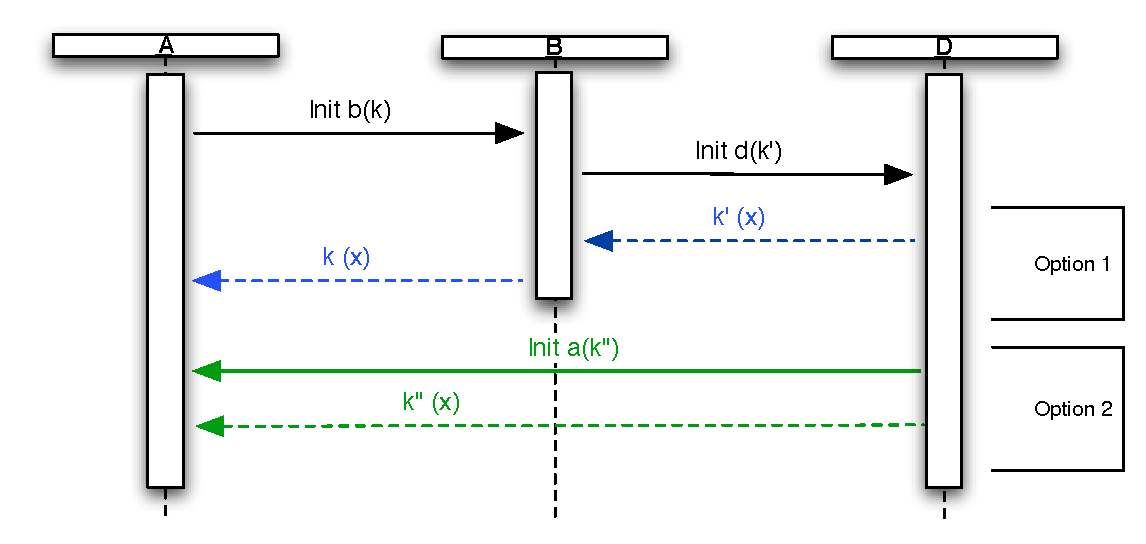
\includegraphics[width=\textwidth]{ServiceSynch}
    \end{center}
    \caption{Diagram of a partial specification.}
    \label{Logic4Struct:fig:diagram}
  \end{myfigure}

  \begin{align}
    C_1 & = \init{A}{B}{b}{k} \pfx \init{B}{D}{d}{k'} \pfx
    \interact{D}{B}{k'}{x}{y_B}\pfx\interact{B}{A}{k}{y_B}{z} \pfx \INACT 
    \label{Logic4Struct:eq:option1} \tag{Option 1} \\
    C_2 & = \init{A}{B}{b}{k} \pfx \init{B}{D}{d}{k'} \pfx
     \init{D}{A}{a}{k''}\pfx \interact{D}{A}{k''}{x}{z} \, \pfx \INACT \, .
     \label{Logic4Struct:eq:option2} \tag{Option 2}
  \end{align}
  We argue that, under the point of view of $A$, both options are
  sufficiently good if, after an initial interaction with $B$ is
  established, there is an eventual response that binds variable
  $z$. Such a property can be expressed by the \GL formula:
  \begin{equation*}
    \exists X,{k''}\pfx \langle\initF{A}{B}{a(k)} \rangle
    \may \Big(\langle \comF{X}{A}{k''}\rangle (z@A=x@D) \Big) \pfx \endT \, .
  \end{equation*}
  Notice that both the choreographies (\ref{Logic4Struct:eq:option1}) and
  (\ref{Logic4Struct:eq:option2}) \emph{satisfy} the partial specification
  above. This will be clear in Section~\ref{Logic4Struct:logic-assertions} where we
  introduce the semantics of logic.

  Also note that a third option for the protocol at hand is to use
  \emph{delegation} (the ability of communicating session keys to
  third participants not involved during session initiation). However,
  the current version of the global calculus does not feature such an
  operation and we leave it as future work.
\end{example}

\begin{example}[Connectedness]
  The work in \cite{carbone7scc} proposes a set of criteria for
  guaranteeing a safe end-point projection between global and local
  specifications (note that the choreography in the previous example
  does not respect such properties). Essentially, a valid global
  specification have to fulfil three different criteria, namely
  Connectedness, Well-threadedness and Coherence.  It is interesting
  to see that some of this criteria relate to global and local
  causality relations between the interactions in a choreography, and
  can be easily formalised as properties in the choreography logic
  here presented. Below, we consider the notion of connectedness and
  leave the other cases as future work. Connectedness dictates a
  global causality principle among interactions. If $A$ initiates any
  action (say sending messages, assignment, etc) as a result of a
  previous event (e.g. message reception), then such a preceding event
  should have taken place at $A$. In the following, let
  $\mathsf{Interact}(A,B)\phi$ be a predicate which is true whenever
  $\langle\ell\rangle\phi$ holds for some $\ell$ with an interaction
  from $A$ to $B$.  Connectedness can then be specified as follows:
  \begin{equation*}
    \forall A,B\pfx
    []
    \Big(
    \mathsf{Interact}(A,B)\true \Rightarrow {}  
    \exists C\pfx 
    \big(\mathsf{Interact}(A,B)\mathsf{Interact}(B,C)\true
    \lor 
    \mathsf{Interact}(A,B)\neg\exists\ell\langle\ell\rangle\true\big)
    \Big) \, . 
  \end{equation*}
%  {\bf Someone: to relate to Dimitris notion of connectedness.}
\end{example}

\subsection{Semantics}\label{Logic4Struct:logic-assertions}

\begin{myfigure}{t!}
  \centering
  \begin{displaymath}
    \begin{array}{lcl}
      \chor\ |=_\sigma \endF & \defSym & \chor \equiv \INACT 
      \\
      \chor\ |=_\sigma (e_1@A = e_2@B) & \defSym & \sigma(e_1@A)\Downarrow v\text{ and }\sigma(e_2@B)\Downarrow v 
      \\
      \chor\ |=_{\sigma}\actionF{ \ell}\phi&\defSym &  (\sigma,\chor)\action{\ell}(\sigma',\chor')\text{ and }\chor'|=_{\sigma'} \phi
      \\
      \chor\ |=_\sigma \phi\land\chi&\defSym &\chor|=_\sigma \phi \text{ and }\chor|=_\sigma \chi 
      \\
      \chor\ |=_\sigma \neg \phi & \defSym & \chor \not |=_\sigma \phi     
      \\
      \chor\ |=_\sigma \exists\var\pfx\phi & \defSym & \chor |=_\sigma \phi[w/\var]
      \text{ (for some appropriate $w$)}
      \\
      \chor\ |=_\sigma \may \phi & \defSym & (\sigma,\chor) \action{}^*(\sigma',\chor') \text{ and } \chor' |=_{\sigma'} \phi
      \\
      \chor\ |=_\sigma \phi \pp \chi & \defSym & \chor\ \equiv\ \chor_1\pp \chor_2 \text{ such that }
      \chor_1 |=_\sigma\phi \text{ and } \chor_2 |=_\sigma \chi
      % C\ |=_\sigma \nextOp \phi & \iff &
      % (\sigma, C) --> (\sigma', C')  \text{ and } C' |=_{\sigma'} \phi
      % \\
      % C\ |=_\sigma \new{k} \phi & \defSym & C \equiv \new{k} C' \text{ and }
      % C' |=_\sigma \phi 
      % \\
      % C\ |=_\sigma \phi \wand \chi & \iff & \forall C_1\pfx C \pp
      % C_1\text{well typed and } C_1 |=_\sigma \phi \text{ implies }C \pp C_1
      % |=_\sigma \chi\quad
      % \chor |=_\sigma \mu X\pfx \phi& \defSym & \chor = {\sf fix}\; \lambda \; f. \lambda \vec{v}. \phi[X / f][ \vec{x} / \vec{v}]
    \end{array}
  \end{displaymath}
  \caption{Assertions of the Choreography Logic}
  \label{Logic4Struct:table:global:assertions}
\end{myfigure}


We now give a formal meaning to the assertions introduced above with
respect to the semantics of the global calculus introduced in the
previous section. In particular, we introduce the notion of
satisfaction.  We write $\chor |=_\sigma \phi$ whenever a state
$\sigma$ and a choreography $\chor$ satisfy a \GL formula $\phi$.  The
relation $|=_\sigma$ is defined by the rules given in
Figure~\ref{Logic4Struct:table:global:assertions}.  In the
$\exists\var\pfx\phi$ case, $w$ should be an appropriate value
according to the type of $\var$, e.g., a participant if $\var$ is a
participant placeholder. Finally, $\sigma(e_1 @ A) \Downarrow$ denotes
the evaluation in the store $\sigma$ of a closed expression $e_1$ in
the participant $A$ with result $v$.

\begin{definition}[Satisfiability, Validity and Logical Equivalence in
  GL]\
  \begin{itemize}
  \item A formula $\phi$ is \emph{satisfiable} if there exists some
    configuration under which it is true, that is, $\chor |=_\sigma
    \phi$ for some $(\chor,\sigma)$.
  \item A formula $\phi$ is \emph{valid} if it is true in every
    configuration, that is, $\chor |=_\sigma \phi$ for every
    $(\chor, \sigma)$.
  \item A formula $\chi$ is a \emph{logical consequence} of a formula
    $\phi$ (or $\phi$ \emph{logically implies} $\chi$), denote with
    an abuse of notation as $\phi |= \chi$, if every configuration
    $(\chor,\sigma)$ that makes $\phi$ true also makes $\chi$ true.
  \item We say that a formula $\phi$ is \emph{logical equivalent} to
    a formula $\chi$, written $\phi \logicEquiv \chi$, if $\phi |= \chi$ iff
    $\chi |= \phi$.
    \item Given a set of formulae $\Phi$ and $\logicEquiv$, the
      equivalence class of $\phi \in \Phi$ is the subset of all
      elements in $\Phi$ such that are logically equivalent to $\phi$:
      \[
      [ \phi ] = \{ x \in \Phi | x \logicEquiv \phi \}
      \]
  \end{itemize}
\end{definition}

%\CommentHugo{ Define the list of formula equivalences for the
%Global Logic, otherwise it is difficult to know when two formulas
%represent the same.}
%
%\begin{proposition}%[Properties of $[ \phi ]$]
%  It holds that:
%     \begin{enumerate}
%       \item $\phi \in [ \phi ] $.
%        \item For any two equivalence classes $[ \phi ], [ \chi ]$, either
%          $[ \phi ]=[ \chi ]$ or $[ \phi ]$ and $[ \chi ]$ are
%          disjoint.
%          \item The set of all equivalence classes of $\Phi$ form a
%            partition of $\Phi$.
%            \item $\chi \logicEquiv \phi$ iff $[ \chi ] = [ \phi ]$.
%       \end{enumerate}
%
%\begin{proof}
%TBD
%\end{proof}
%\end{proposition}

%%% Local Variables: 
%%% mode: latex
%%% TeX-master: "../Thesis"
%%% End: 
